\ctitle{Definitions}

\paragraph{Convexity}\index{Convexity} Used to describe a special case of the general constrained optimization problem in which
\begin{itemize}[nolistsep,noitemsep]
    \item The objective function is convex
    \item The equality constraint functions $c_i(\cdot)$, $i \in \mathcal{E}$ are linear, and
    \item The inequality constraint functions$c_i(\cdot)$, $i \in \mathcal{I}$ are concave
\end{itemize}

\paragraph{LICQ}\index{LICQ} (Linear Independence Constraint Qualification) Given the point $x$ and the active set $\mathcal{A}(x)$, we say that the LICQ holds if the set of active constraint gradients $\nabla c_i (x), \: i \in \mathcal{A}(x)$ is linearly independent.

\paragraph{Search directions} \index{Search directions} Several approaches to line search directions can be used:

\hskip-0.5cm
\begin{tabularx}{\linewidth}{X X}
	\textbf{Method} & \textbf{Formula}\\
	\hline
	Steepest descent & $p_k=-\nabla f_k$\\
	Newton direction & $p_k^N=-(\nabla^2 f_k)^{-1}\nabla f_k$ \\
	Quasi-Newton direction & $p_k=-B_k^{-1}\nabla f_k$ \\
	\quad SR1(Symmetric-rank-one) & For updating $B_k$\\
	\quad BFGS & \\
	% Could add Conjugate gradient line
\end{tabularx}

\paragraph{The Wolfe conditions} \index{The Wolfe conditions}
Are used in line-search methods to decide if the decrease in the objective function is sufficient.
\begin{equation}
    f(x_k+\alpha p_k) <= f(x_k) + c_1 \alpha \nabla f_k^T p_k
\end{equation}

There is also a second Wolfe condition, but we don't need it if we use backtracking.

\paragraph{Merit functions}\index{Merit functions} SQP methods often use merit functions to decide whether a trail step should be accepted. In line search methods, the merit function controls the size of the step.
\begin{equation}
    \begin{split}
        l_1\text{:} \quad \phi_1(x;\mu) &= f(x) + \mu \sum_{i \in \mathcal{E}} |c_i(x)| + \mu \sum_{i \in \mathcal{I}} [c_i(x)]^-\\
        %l_2\text{:} \quad \phi_2(x;\mu) &= f(x) + \mu || c(x) ||_2
    \end{split}
\end{equation}

Notation: $[z]^- = \text{max}\{0, -z\}$

The positive scalar $\mu$ is the penalty parameter, which determines the weight that we assigned to constraint satisfaction relative to minimization of the objective.

\textit{Exact merit function:} A merit function $\phi(x; \mu)$ is exact if there is a positive scalar $\mu^*$ such that for any $\mu > \mu^*$, any local solution of the nonlinear programming problem is a local minimizer of $\phi(x; \mu)$. 

\paragraph{Maratos effect}\index{Maratos effect} The phenomenon where a merit function prevents rapid convergence because steps that make good progress toward a solution are rejected.

\begin{figure}[H]
	\centering
	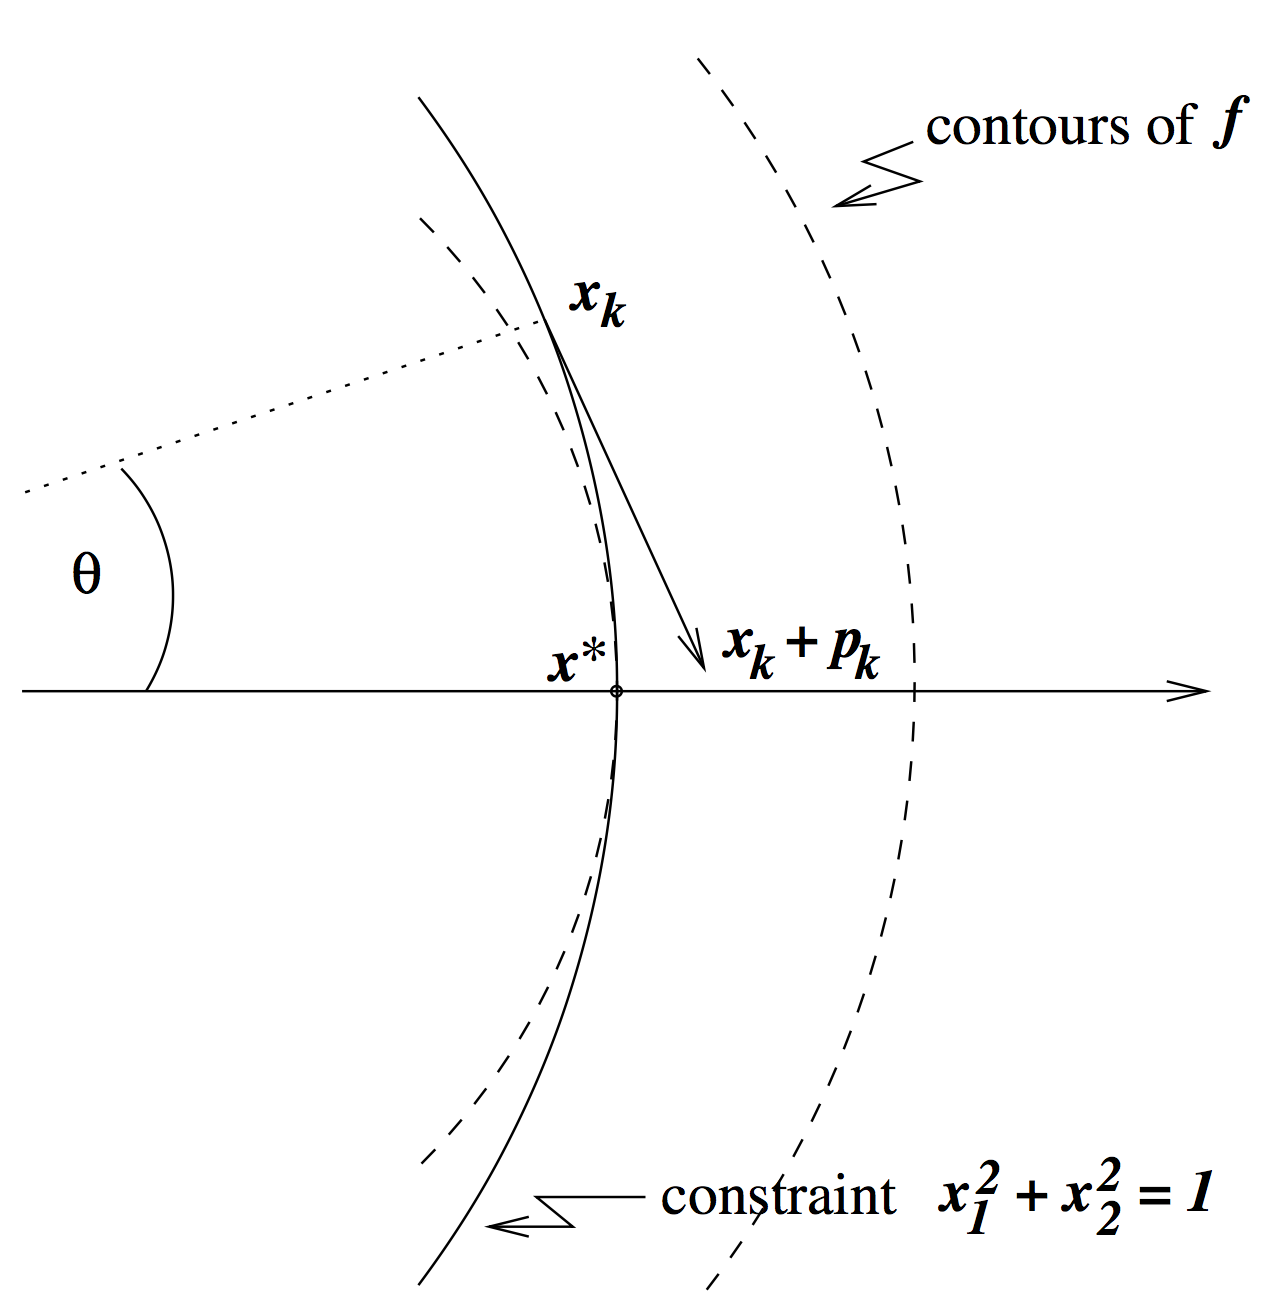
\includegraphics[width=0.3\textwidth]{images/maratos_effect}
	\caption{Maratos Effect}
	\label{fig:maratos_effect}
\end{figure}

% Definitions in course handout:
\paragraph{Model predictive control}\index{model predictive control} (MPC) A form of control in which the current control action is obtained by solving, at each sampling instant, a finite horizon open-loop optimal control problem, using the current state of the plant as the initial state; the optimization yields an optimal control sequence and the first control in this sequence is applied to the plant.

\paragraph{Full-space VS Reduced-space formulation} \index{Full-space formulation} \index{Reduced-space formulation}
 \begin{itemize}[nolistsep,noitemsep]
     \item In full-space optimization, we include all inputs and all states in our objective function. The number of optimization variables is $\#\mathrm{steps} \cdot (\#\mathrm{states} + \#\mathrm{inputs})$.
     \item In reduced-space optimization, we remove the states from the objective function by replacing them using the model ($x_{t+1} = A_t x_t + B_t u_t$). The number of optimization variables is $\#\mathrm{steps} \cdot \#\mathrm{inputs}$.
 \end{itemize}
 
\hskip-0.5cm
\begin{tabularx}{\linewidth}{X X X}
	& \textbf{Pros} & \textbf{Cons}\\
	\hline
	\textbf{Full-space} & Often sparsity in matrices & Many variables\\
	\textbf{Reduced-space} & Less variables & Normally dense matrices
\end{tabularx}

\paragraph{Stabilizability} \index{Stabilizability}
Tells us that we must be able to influence all unstable modes. Important for LQGC.

\paragraph{Detectability}\index{Detectability}
A milder form of observability. This implies that an
observable system always is detectable. The opposite is however not
necessarily true. Important for LQGC